\chapter[Relatório Lidar]{Relatório Lidar}
\begin{enumerate}
\item \textbf{Descrição}
O Lidar funciona com a emissão de um laser que será refletido por um objeto (o que se deseja medir a distância) e depois detectado fazendo uso das propriedades da luz para se obter as informações desejadas. Seu funcionamento é parecido com o do radar, porém com pulsos de laser ao invés de ondas de rádio.

Uma grande desvantagem do Lidar é que sua utilização não é efetiva em climas adversos como chuva e neblina devendo ser utilizado em boas condições climáticas, na maioria das aplicações com Lidar as detecções são feitas de noite onde seu desempenho costuma ser melhor.

\item \textbf{Especificações DO LIDAR}

O Lidar utilizado será o HDL-64E da Velodyne que possui uma alta definição e consegue captar uma distância de até 120 m com alta resolução.

\begin{table}
\begin{tabular}{|p{8cm}|p{8cm}|}
\hline
Sensor & 64 laser/detectores\\ 
& Campo de visão de 360 graus (azimute)\\ 
& Resolução angular de 0,08 graus (azimute)\\  
& Campo de visão na vertical de 26,8 graus (elevação) de +2 até -24,8 com 64 subdivisões angulares igualmente espaçadas (aproximadamente 0,4)\\  
& < 2 cm de precisão de distância\\  
& 5-15 Hz de atualização do campo de visão (escolhido pelo usuário)\\  
& 50 metros de alcance para pavimento (aproximadamente 0,10 de refletividade)\\  
& 120 metros de alcance para carros e folhagem (aproximadamente 0,80 de refletividade)\\  
& > 1,3 M pontos por segundo\\ 
& Temperatura de operação – 10 a 50 ºC\\  
& Temperatura de armazenamento - 10 a 80 ºC\\  \hline
Laser & Classe 1 – seguro para os olhos\\ 
& Comprimento de onda de 905 nm\\ 
& Aproximadamente 10 ns de tamanho do pulso\\ 
& Potência do laser dinâmica para um maior alcance dinâmico\\ \hline
Maquinal & 15 V $\pm$ 1,5 V @ 4 amps\\ 
& < 29 lbs\\ 
& Cilindro de 10’’ de altura e de 8’’ de raio\\ 
& Taxa de rotação de 300 RPM – 900 RPM (escolhido pelo usuário)\\ 
& Proteção ambiental IP67\\ \hline
Saída & Pacotes Ethernet 100 MBPS UDP \\ \hline
\end{tabular}
\end{table}

Design do produto de acordo com a Figura \ref{fig:design_lidar}

\begin{figure}[h]
  \centering
  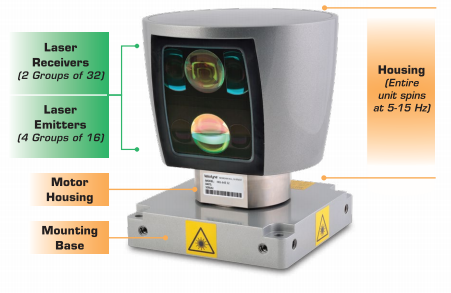
\includegraphics[width=400px, scale=1]{figuras/design_lidar}
  \caption{Design do Lidar}
\label{fig:design_lidar}
\end{figure}

Imagem obtida com esse equipamento

\begin{figure}[h]
  \centering
  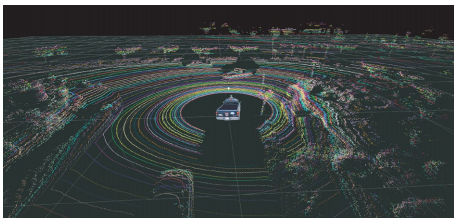
\includegraphics[width=400px, scale=1]{figuras/img_lidar}
  \caption{Imagem do equipamento LIDAR}
\label{fig:img_lidar}
\end{figure}
\end{enumerate}
